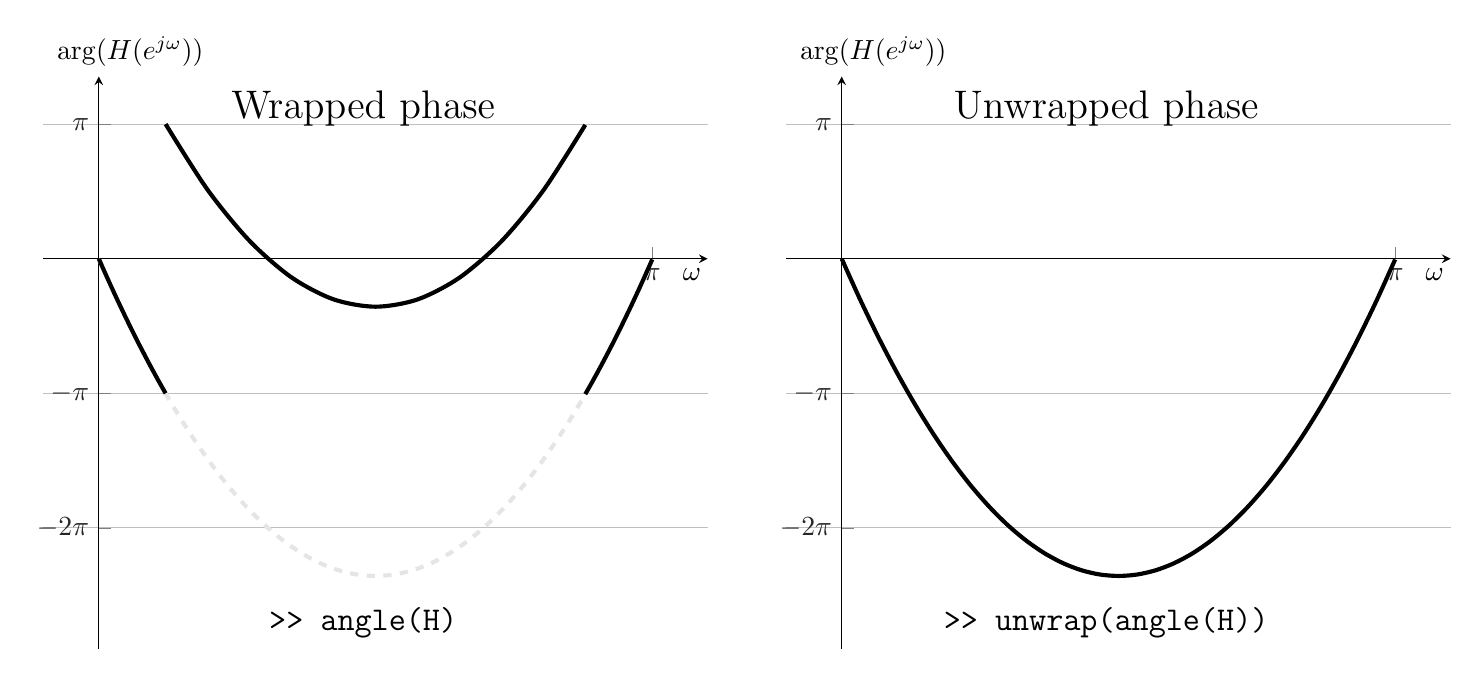
\begin{tikzpicture}
\begin{axis}[
name=plot1,
axis lines*=middle,
enlargelimits = true, clip=true,
scale only axis,
axis line style={->,>=stealth},
xlabel={$\omega$},
ylabel={$\arg(H(e^{j\omega}))$},
every axis x label/.style={
	at={(ticklabel* cs:1)},
	xshift=-0.2cm,
	anchor=north,
},
every axis y label/.style={
	at={(ticklabel* cs:1)},
	xshift=0.4cm,
	%yshift=0.35cm,
	anchor=south,
},
every outer x axis line/.append style={white!15!black},
every x tick label/.append style={font=\color{white!15!black}},
xmin=0, xmax=3.14,
ymin=-8, ymax=3.14,
xtick={0, 3.14},
xticklabels ={$0$, $\pi$},
ytick={3.14, -3.14, -6.28},
yticklabels={$\pi$, $-\pi$, $-2\pi$},
ymajorgrids,
every outer y axis line/.append style={white!15!black},
every y tick label/.append style={font=\color{white!15!black}},
legend style={draw=white!15!black,fill=white,legend cell align=left}]
\addplot [smooth, dashed, black!10, line width=1.5pt, forget plot, domain=0:3.14, samples=31] {3*x*(x-pi)};
\addplot [smooth, black, line width=1.5pt, forget plot, domain=0:0.379, samples=11] {3*x*(x-pi)};
\addplot [smooth, black, line width=1.5pt, forget plot, domain=0.379:2.76, samples=11] {2*pi + 3*x*(x-pi)};
\addplot [smooth, black, line width=1.5pt, forget plot, domain=2.76:3.14, samples=11] {3*x*(x-pi)};


\node at (axis cs: 1.5, 3.5) {\Large Wrapped phase};
\only<2|handout:1>{\node at (axis cs: 1.5, -8.5) {\large \texttt{>> angle(H)}};}
\end{axis}

\begin{axis}[
name=plot2,
at= (plot1.east), anchor=west,
xshift=1cm,
axis lines*=middle,
enlargelimits = true, clip=true,
scale only axis,
axis line style={->,>=stealth},
xlabel={$\omega$},
ylabel={$\arg(H(e^{j\omega}))$},
every axis x label/.style={
	at={(ticklabel* cs:1)},
	xshift=-0.2cm,
	anchor=north,
},
every axis y label/.style={
	at={(ticklabel* cs:1)},
	xshift=0.4cm,
	%yshift=0.35cm,
	anchor=south,
},
every outer x axis line/.append style={white!15!black},
every x tick label/.append style={font=\color{white!15!black}},
xmin=0, xmax=3.14,
ymin=-8, ymax=3.14,
xtick={0, 3.14},
xticklabels ={$0$, $\pi$},
ytick={3.14, -3.14, -6.28},
yticklabels={$\pi$, $-\pi$, $-2\pi$},
ymajorgrids,
every outer y axis line/.append style={white!15!black},
every y tick label/.append style={font=\color{white!15!black}},
legend style={draw=white!15!black,fill=white,legend cell align=left}]
\addplot [smooth, black, line width=1.5pt, forget plot, domain=0:3.14, samples=31] {3*x*(x-pi)};

\node at (axis cs: 1.5, 3.5) {\Large Unwrapped phase};
\only<2|handout:1>{\node at (axis cs: 1.5, -8.5) {\large \texttt{>> unwrap(angle(H))}};}

\end{axis}

\end{tikzpicture}